\documentclass[border=3mm]{standalone}
% Shared figure palette and OFL font setup. Compile from docs/assets/.
\usepackage{fontspec}
\setmainfont{public-sans-regular.ttf}[Path=fonts/,BoldFont=public-sans-semibold.ttf]
\setsansfont{public-sans-regular.ttf}[Path=fonts/,BoldFont=public-sans-semibold.ttf]
\setmonofont{ibm-plex-mono.ttf}[Path=../../app/public/fonts/,Scale=MatchLowercase]
\usepackage{xcolor,tikz,fontawesome5}
\usetikzlibrary{positioning,calc,arrows.meta}
\definecolor{ink}{HTML}{14110F}
\definecolor{vellum}{HTML}{EDE3CF}
\definecolor{vermilion}{HTML}{B8322A}
\definecolor{verdigris}{HTML}{3E8E7E}
\definecolor{gold}{HTML}{C9A24A}
\definecolor{navy}{HTML}{1F3A5F}
\definecolor{oiblue}{HTML}{0072B2}
\definecolor{oigreen}{HTML}{009E73}
\definecolor{oiverm}{HTML}{D55E00}
\definecolor{grey}{HTML}{555555}
\newlength{\colw}\setlength{\colw}{62mm}
\newcommand{\figbody}{\fontsize{20}{25}\selectfont}
\newcommand{\figtitle}{\fontsize{22}{26}\selectfont\bfseries}
\newcommand{\figlegend}{\fontsize{16}{20}\selectfont}
\newcommand{\cardtext}[4]{%
  \begin{minipage}[c][29mm][t]{6mm}\vspace{1mm}\centering{\fontsize{16}{20}\selectfont\color{#1}#2}\end{minipage}\hspace{1mm}%
  \begin{minipage}[c][29mm][t]{\dimexpr\colw-14mm\relax}\raggedright\hyphenpenalty=10000\exhyphenpenalty=10000
  \figbody\color{ink}
  {\figtitle\strut #3}\par\vspace{1.5mm}
  #4\par\end{minipage}}
% The document and circle icons use code; TableSealed uses Font Awesome's ban glyph.
\newcommand{\cardicon}{\tikz[baseline=-1mm]\draw[line width=1pt,rounded corners=.3mm] (0,0) rectangle (4mm,5mm);}
\newcommand{\sealicon}{\tikz[baseline=-1mm]\draw[line width=1.2pt] (0,0) circle (2mm);}
\tikzset{card/.style={draw=#1!55,fill=white,rounded corners=2mm,line width=.7pt,minimum width=\colw-4mm,minimum height=34mm,inner sep=1.5mm,anchor=north west},
link/.style={-{Stealth[length=2.5mm,width=2.3mm]},line width=1.3pt,color=grey}}

\newcommand{\column}[5]{%
  \fill[#2!6,rounded corners=3mm] (#1,0) rectangle ++(\colw,-100mm);
  \fill[#3,rounded corners=3mm] (#1,0) rectangle ++(\colw,-18mm);
  \node[anchor=north west,text=white,font=\fontsize{25}{29}\selectfont\bfseries,align=left] at ($(#1,0)+(3mm,-3mm)$) {#4\hspace{2mm}#5};}
\begin{document}
\begin{tikzpicture}
\column{0mm}{navy}{navy}{1}{Seal}
\column{68mm}{oiverm}{oiverm!75!black}{2}{Plea}
\column{136mm}{oiblue}{oiblue}{3}{Request}
\column{204mm}{oigreen}{oigreen!65!black}{4}{Callback}
\column{272mm}{navy}{navy}{5}{Verify}
\node[card=navy] (draft) at (2mm,-22mm) {\cardtext{navy}{\cardicon}{Ruling}{DC + four\\outcomes}};
\node[card=navy] (seal) at (2mm,-62mm) {\cardtext{navy}{\sealicon}{Seal}{Table\\frozen}};
\node[card=oiverm] (plea) at (70mm,-22mm) {\cardtext{oiverm}{\cardicon}{Keeper}{Agrees to\\lower DC}};
\node[card=oiverm] (refusal) at (70mm,-62mm) {\cardtext{oiverm}{\faBan}{TableSealed}{Plea stays\\in the logs}};
\node[card=oiblue] (request) at (138mm,-22mm) {\cardtext{oiblue}{\cardicon}{Request}{Scoped to\\this check}};
\node[card=oiblue] (once) at (138mm,-62mm) {\cardtext{oiblue}{\sealicon}{One roll}{Only once\\per check}};
\node[card=oigreen] (callback) at (206mm,-22mm) {\cardtext{oigreen}{\cardicon}{Callback}{VRF sends\\randomness}};
\node[card=oigreen] (resolve) at (206mm,-62mm) {\cardtext{oigreen}{\sealicon}{Resolve}{d20 picks\\the row}};
\node[card=navy] (rpc) at (274mm,-22mm) {\cardtext{navy}{\cardicon}{RPC reads}{Check and\\TX records}};
\node[card=navy] (verify) at (274mm,-62mm) {\cardtext{navy}{\sealicon}{Re-check}{Seal, VRF\\and d20}};
\foreach \p/\q in {draft/seal,request/once,callback/resolve,rpc/verify}{\draw[link] ([yshift=-1mm]\p.south)--([yshift=1mm]\q.north);}
% The main path bypasses the optional plea. The refusal never rejoins it.
\draw[link] (seal.east) -- ++(3mm,0) |- (135mm,-106mm) |- (request.west);
\draw[link,dashed] ([yshift=6mm]seal.east) -- ++(5mm,0) |- (plea.west);
\draw[link,dashed] ([yshift=-1mm]plea.south) -- ([yshift=1mm]refusal.north);
\draw[link] (request.east) -- (callback.west);
\draw[link] (resolve.east) -- ++(3mm,0) |- (rpc.west);
\fill[black!4,rounded corners=1mm] (0,-113mm) rectangle (334mm,-125mm);
\node[anchor=west,font=\figlegend,text=grey] at (3mm,-119mm) {Solid = turn path.\quad Dashed = optional plea, refused.};
\end{tikzpicture}
\end{document}
